%% A brief test of different estimators of galaxy peculiar velocity
%% Sun Nov 29, 2015
%% Christopher Rooney
\nonstopmode
\documentclass[usenatbib]{mn2e}

%%%%%%%%%%%%%%%%%%%%%%%%%%%%%%%%%%%%%%%%%%%%%%%%%%%%%%%%%%%%%%%%%%%%%%
%% This section is called the preamble, where we can specify which
%% latex packages we required.  Most (but not of all) of the packages
%% below should be fairly standard in most latex documents.  The
%% exception is xspace and the new \latex command, which you probably
%% do not need.
%%%%%%%%%%%%%%%%%%%%%%%%%%%%%%%%%%%%%%%%%%%%%%%%%%%%%%%%%%%%%%%%%%%%%%

%% Bibliography style:
\usepackage{mathptmx}           % Use the Times font.
\usepackage{graphicx}           % Needed for including graphics.
\usepackage{url}                % Facility for activating URLs.
\usepackage{verbatim}           % For verbatiminput command.
\usepackage{booktabs}
%% Set the paper size to be letter, with a 2cm margin 
%% all around the page.
\usepackage{gensymb}

\newcommand{\iu}{{i\mkern1mu}}
\newcommand{\e}{{\mathrm e}}
\usepackage{xspace}
 

\voffset=-0.5truein
\textheight=9.5truein
\textwidth=6.5truein
\voffset=-0.55in
\hoffset=0.06in
\textwidth=6.4in
\textheight=9in
%
\def\gtwid{\mathrel{\raise.3ex\hbox{$>$\kern-.75em\lower1ex\hbox{$\sim$}}}}
\def\ltwid{\mathrel{\raise.3ex\hbox{$<$\kern-.75em\lower1ex\hbox{$\sim$}}}}
\def\lessim{\mathrel{\raise.3ex\hbox{$<$\kern-.75em\lower1ex\hbox{$\sim$}}}}
\def\\{\hfil\break}
\def\ie{{\it i.e.\ }}
\def\eg{{\it e.g.\ }}
\def\etal{{\it et al.\ }}
%\newcommand{\apj}{ApJ}

%Astro Stuff
%some units
\newcommand{\km}{\unit{km}}
\newcommand{\kms}{\unit{km~s\mone}}
\newcommand{\kpc}{\unit{kpc}}
\newcommand{\mpc}{\unit{Mpc}}
\newcommand{\hkpc}{\mamo{h\mone}\kpc}
\newcommand{\hmpc}{\mamo{h\mone}\mpc}
\newcommand{\parsec}{\unit{pc}}
\newcommand{\chisq}{\mamo{\chi^2}}
%
\newcommand{\hr}{\mamo{^{\rm h}}}
\newcommand{\m}{\mamo{^{\rm m}}}
%
\newcommand{\lb}[2]{\mamo{l = #1\arcdeg}, \mamo{b = #2\arcdeg}}
\newcommand{\dlb}[4]{\mamo{l = #1\fdg#2}, \mamo{b = #3\fdg#4}}
\newcommand{\lbapr}[2]{\mamo{l \approx #1\arcdeg}, \mamo{b \approx #2\arcdeg}}
%
\newcommand{\rightascen}{\mbox{R.A.}}
\newcommand{\declin}{\mbox{Dec.}}
\newcommand{\radec}[2]{\mamo{\alpha = #1^{\rm h}}, \mamo{\delta = #2\arcdeg}}
\newcommand{\dradec}[4]{\mamo{\alpha = #1\fh#2}, \mamo{\delta = #2\fdg#4}}
%
\newcommand{\xyz}[3]{($#1$, $#2$, $#3$)}
%
% useful abbreviations
\newcommand{\wrt}{with respect to}
\newcommand{\ebv}{\mbox{$E(B-V)$}}
\renewcommand{\lg}{\mamo{\sb{LG}}}
\newcommand{\cmb}{\mamo{\sb{CMB}}}
\newcommand{\rhat}{\mamo{\hat{\bfv{r}}}}
%
\newcommand{\secref}[1]{Section~\ref{sec:#1}}
\newcommand{\brref}[1]{(equation~\ref{eq:#1})}
%\newcommand{\eqref}[1]{equation~(\ref{eq:#1})}
\newcommand{\Eqref}[1]{Equation~(\ref{eq:#1})}
\newcommand{\figref}[1]{Fig.~\ref{fig:#1}}
\newcommand{\tabref}[1]{Table~\ref{tab:#1}}

\newcommand{\bt}{\mamo{B/T}}
\newcommand{\br}{\mamo{B-R}}
\newcommand{\del}{\mbox{d}}

\newcommand{\aap}{A\&A}
\newcommand{\apj}{ApJ}
\newcommand{\apjl}{ApJL}
\newcommand{\apjs}{ApJ Supp}
\newcommand{\aj}{AJ}
\newcommand{\mnras}{MNRAS}
\newcommand{\pasp}{PASP}
\newcommand{\prd}{Phys Rev D}
\begin{document}

\author{Christopher Rooney}
\date{\today}
\title{Perturbing the Velocity Correlations}
\maketitle

\begin{abstract}
Here the effects of errors in distance are tested on the velocity correlation estimators. Surveys that have been perturbed are tested against surveys that we have ``perfect knowledge'' of. It is found that many features are wiped out by the perturbations.
\end{abstract}

\section{Introduction}
In previous studies, the velocity correlation functions have been computed over known galaxy surveys. Usually, these surveys have large errors in the velocity, and few galaxies ($\approx 4000$). In this paper, we will begin building confidence that velocity correlation information computed with data from the CosmicFlows-2 catalogs are reliable (not error-dominated). To accomplish this, 300 CF2-like surveys are collected from Millennium Simulation galaxies. Several of these surveys are selected and perturbed to better resemble real-life data. The perturbed catalogs can be compared with the perfect catalogs to establish the effects of such large errors on the analysis of the data.

\section{Procedure}
Galaxies were selected from the DeLucia2006a catalog to match the radial distribution of galaxies found in each of the COMPOSITE, CF2-gal and CF2-group catalogs. In each of these surveys, the position, redshift, and peculiar velocities of the galaxies are known with perfect accuracy. Using 100 of these catalogs, the velocity correlation was computed as described by Gorski (YEAR). Then two catalogs were selected from each category (CF2-gal, CF2-group, Composite) at random. The distances to galaxies in all of the selected catalogs were perturbed at random one hundred times (with two different error sizes), producing 1200 additional catalogs. 

To perturb the catalogs, the following method was used. The perfectly-known distance data was converted to a distance modulus. The distance modulus was perturbed by a normal distribution with standard-deviations equal to either 0.1 or 0.2 times the distance modulus. The new distance was computed simply by taking the exponential function of the perturbed distance modulus, and the new peculiar velocity was computed using the unbiased estimator described in Feldman (2015).

\section{Results}
Figure~\ref{fig:perf-kms} shows the perfect velocity correlation as a function of redshift. This exact plot came from the COMPOSITE sample, but it is representative of all the others. For comparison, Figure~\ref{fig:imperf-kms} is the correlation as a function of redshift after perturbing one of the surveys 100 times with relative errors in the distance modulus equal to 0.2. It appears that it is completely error-dominated now, with everything consistent with zero. That is probably not due to the individual survey chosen to perturb, because Figure~\ref{fig:single} shows a plot of the single survey, and it appears to have more in common with Figure~\ref{fig:perf-kms} than Figure~\ref{fig:imperf-kms}. These patterns are seen in all combinations of perfect and imperfect surveys tested.
\begin{figure}
  \begin{center}
  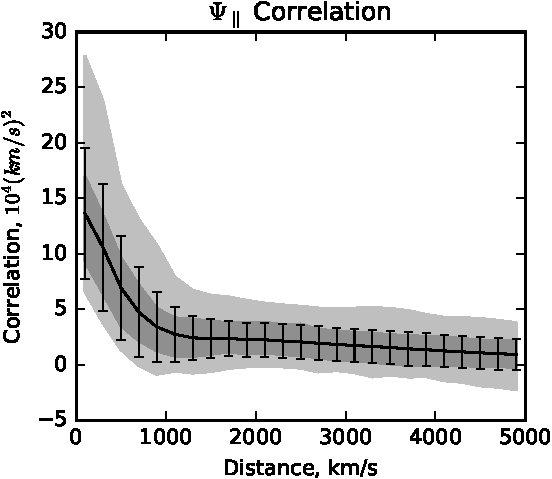
\includegraphics[scale=0.75]{psipar-perf-kms.pdf}
  \end{center}
\caption{\small
The perfect velocity correlation as a function of redshift. The light grey contours represent the 95th percentile, and the dark grey contours represent the 68th percentile. The error bars are one standard deviation. This plot was generated using the 100 ``perfect knowledge'' COMPOSITE surveys.
}
\label{fig:perf-kms}
\end{figure}
\begin{figure}
  \begin{center}
  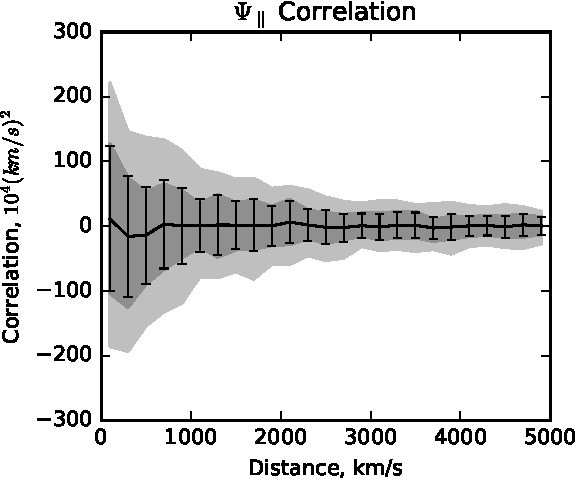
\includegraphics[scale=0.75]{psipar-pert-0,2-comp29-kms.pdf}
  \end{center}
\caption{\small
The velocity correlation as a function of redshift, of 100 perturbed COMPOSITE surveys. The contours and error bars in this plot are the same as in Fig.~\ref{fig:perf-kms}.
}
\label{fig:imperf-kms}
\end{figure}
\begin{figure}
  \begin{center}
  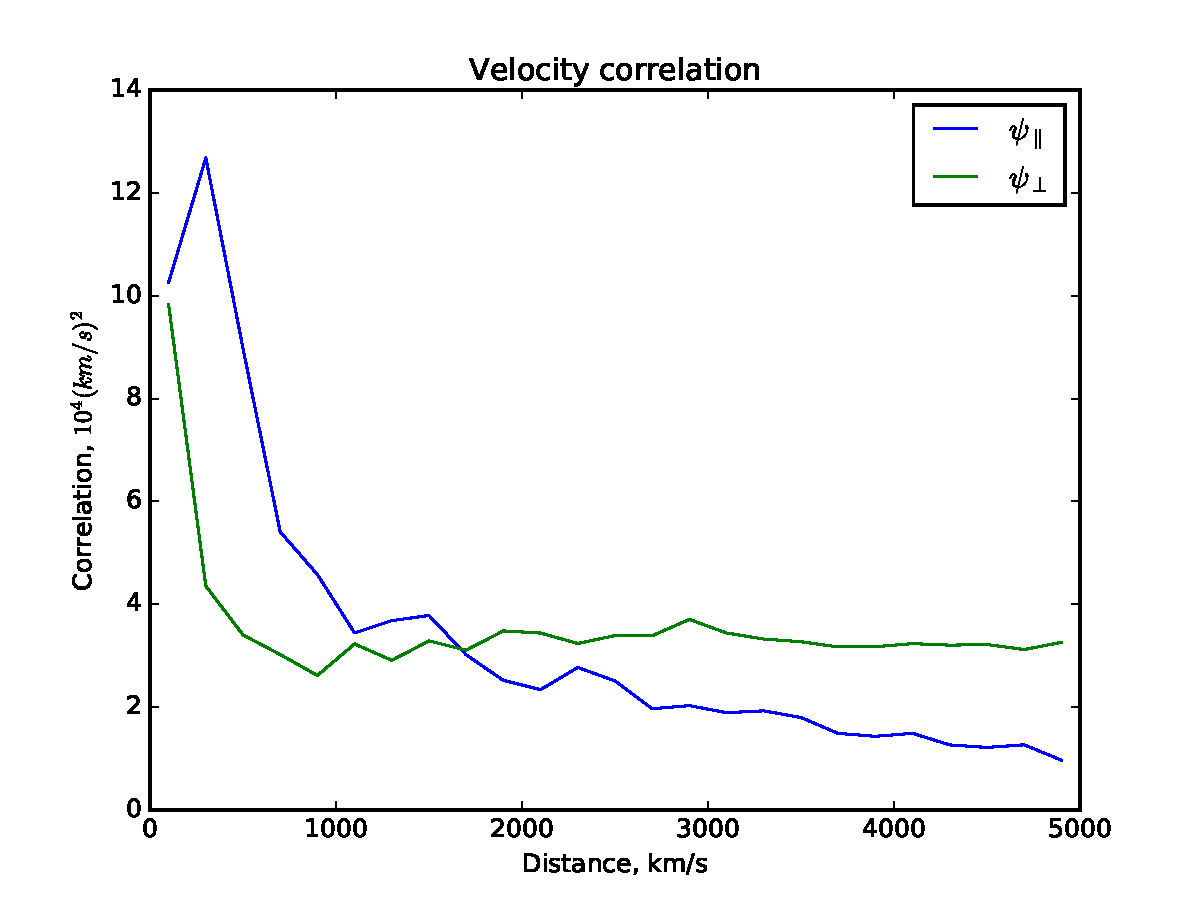
\includegraphics[scale=0.4]{single-vcorr-composite1.pdf}
  \end{center}
\caption{\small
The perfect velocity correlation as a function of redshift. This plot uses only the one perfect COMPOSITE survey used to generate all of the perturbed surveys in Fig.~\ref{fig:imperf-kms}.
}
\label{fig:single}
\end{figure}

A similar situation is found when dealing with correlations as a function of distance, although in this case the dominant feature in the perfect data was a negative slope, which is still seen in the perturbed data. The perfect data is shown in Figure~\ref{fig:perf-mpc}. In the perturbed plots, the scale is wildly different. Instead of the velocity correlation staying between -5 and 25 like it does with the perfect data, it tends to be much more exaggerated in the perturbed data. Figure ~\ref{fig:pert-mpc} may not be the best plot for the job, but it works. In that plot, correlation decreases from -100 to -600. Again, similar features are seen in other combinations of perfect and imperfect datasets.

\begin{figure}
  \begin{center}
  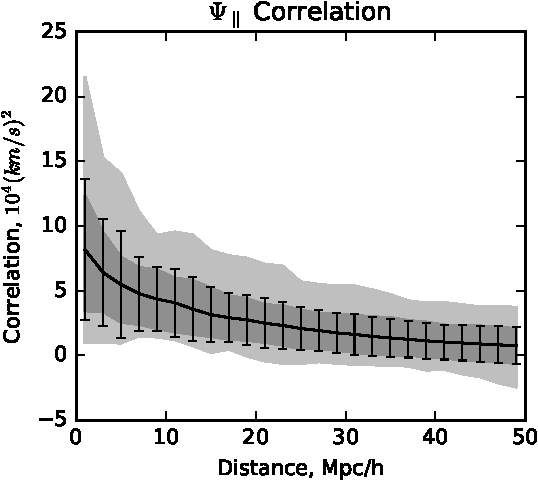
\includegraphics[scale=0.75]{psipar-perf-Mpch.pdf}
  \end{center}
\caption{\small
The perfect velocity correlation as a function of distance. This plot uses only the one perfect COMPOSITE survey used to generate all of the perturbed surveys in Fig.~\ref{fig:imperf-kms}.
}
\label{fig:perf-mpc}
\end{figure}
\begin{figure}
  \begin{center}
  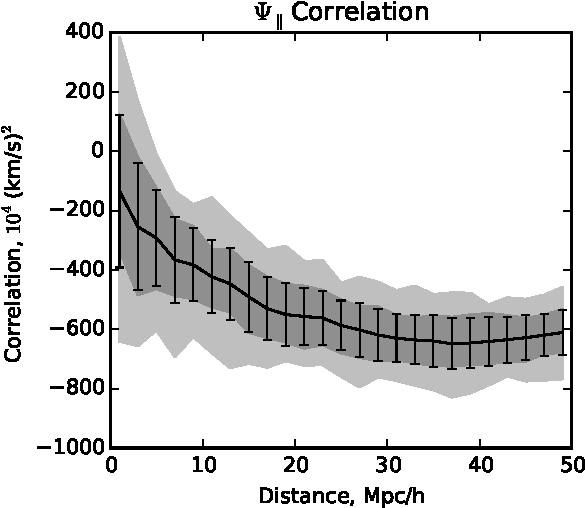
\includegraphics[scale=0.75]{psipar-pert-0,2-comp1-mpc.pdf}
  \end{center}
\caption{\small
One plot of the imperfect velocity correlation as a function of distance. The contours and error bars in this plot are the same as in Fig.~\ref{fig:perf-kms}. Note that the scaling is wildly exaggerated from that in Fig~\ref{fig:perf-mpc}.
}
\label{fig:pert-mpc}
\end{figure}

\section{Discussion}
The perturbed dataset definitely appears to be error-dominated. Whereas there was a clear boost to correlation at small scales when using redshift as distance in the perfect data, there were no such clear features when using the perturbed data. There was still a clear negative slope in the perturbed surveys when using distance as distance, the scale was completely different ($20 \cdot 10^4$ (km/s)$^2$  as opposed to $2500 \cdot 10^4$ (km/s)$^2$). I'm not entirely sure what this means, but it doesn't seem good for being able to extract meaningful information from real surveys. 

\section{Future Work}
One thing I could try would be to turn on weighting, and weight galaxies by their errors. This way galaxies with huge errors would have less effect on the end result. We could see where this takes us.

%%%%%%%%%%%%%%%%%%%%%%%%%%%%%%%%%%%%%%%%%%%%%%%%%%%%%%%%%%%%%%%%%%%%%%
%% Finally we specify the format required for our references and the
%% name of the bibtex file where our references should be taken from.
%%%%%%%%%%%%%%%%%%%%%%%%%%%%%%%%%%%%%%%%%%%%%%%%%%%%%%%%%%%%%%%%%%%%%%
\bibliographystyle{mn2e}
\bibliography{paper}
\end{document}

%%%%%%%%%%%%%%%%%%%%%%%%%%%%%%%%%%%%%%%%%%%%%%%%%%%%%%%%%%%%%%%%%%%%%%
%% The end.
%%%%%%%%%%%%%%%%%%%%%%%%%%%%%%%%%%%%%%%%%%%%%%%%%%%%%%%%%%%%%%%%%%%%%%
